\subsection{UC3 – Proposta profilo}
\begin{center}
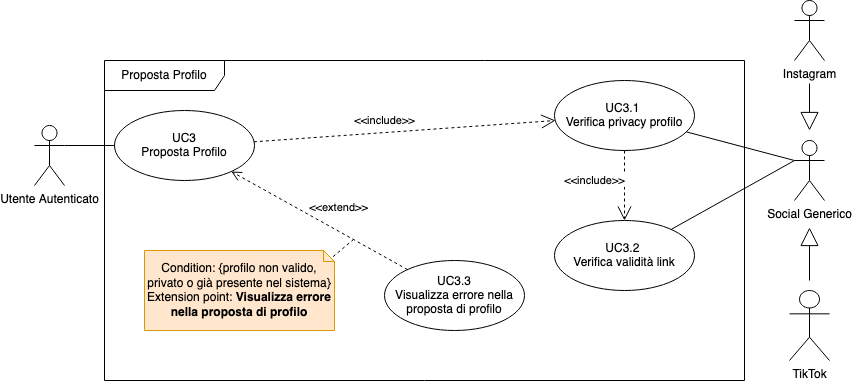
\includegraphics[scale=0.5]{UC_images/UC3.png}
\end{center}
\begin{itemize}
    \item \textbf{Attore primario}: Utente autenticato.
    \item \textbf{Precondizione}: Il sistema possiede una lista di profili social da cui effettuare il crawling dei dati.
    \item \textbf{Postcondizione}: Alla lista di profili da cui effettuare il crawling viene aggiunto il profilo indicato dall’utente e tutti i profili pubblici presenti nella lista amici del profilo suggerito.
    \item \textbf{Scenario principale}: 
    \begin{enumerate}
        \item L'utente autenticato accede al sistema;
        \item L’utente seleziona la funzionalità suggerisci un profilo;
        \item L’utente inserisce il link valido ad un profilo instagram o tiktok pubblico.
    \end{enumerate}
    \item \textbf{Estensioni}:
    \begin{itemize}
        \item Nel caso in cui l’utente inserisce un link non valido:
        \begin{enumerate}
            \item Il link non viene inserito nella lista;
            \item Viene visualizzato un messaggio di errore nella proposta di profilo (UC3.3 §);
            \item Viene fornita all’utente la possibilità di modificare il link.
        \end{enumerate}
        \item Nel caso in cui l’utente inserisce il link ad un profilo privato:
        \begin{enumerate}
            \item Il link non viene inserito nella lista;
            \item Viene visualizzato un messaggio di errore nella proposta di profilo (UC3.3 §).
        \end{enumerate}
        \item Nel caso in cui viene inserito un link valido ad un profilo pubblico già presente nel sistema:
        \begin{enumerate}
            \item Il link non viene inserito nella lista.
        \end{enumerate} 
    \end{itemize}
    \item Inclusioni:
    \begin{enumerate}
        \item Verifica privacy profilo (UC3.1).
    \end{enumerate}
\end{itemize}

\subsection{UC3.1 – Verifica privacy profilo}
\begin{itemize}
    \item \textbf{Attore primario}: Utente autenticato.
    \item \textbf{Attore secondario}: Social generico.
    \item \textbf{Precondizione}: L’utente ha richiesto l’aggiunta di un profilo social fornendone il link.
    \item \textbf{Postcondizione}: Il sistema sa se il profilo suggerito è pubblico o privato.

    \item \textbf{Scenario principale}: 
    \begin{enumerate}
        \item Il sistema chiede al social in questione se il profilo proposto è pubblico o privato;
        \item Il social in questione invia una risposta dicendo se il profilo è pubblico o privato.
    \end{enumerate}

    \item \textbf{Inclusioni}:
    \begin{enumerate}
        \item Verifica validità link (UC3.2 §).
    \end{enumerate}
\end{itemize}

\subsection{UC3.2 – Verifica validità link}
\begin{itemize}
    \item \textbf{Attore primario}: Utente autenticato.
    \item \textbf{Attore secondario}: Social generico.
    \item \textbf{Precondizione}: L’utente ha richiesto l’aggiunta di un profilo social fornendone il link.
    \item \textbf{Postcondizione}: Il sistema sa se il link fornito è valido.

    \item \textbf{Scenario principale}: 
    \begin{enumerate}
        \item Il sistema chiede al social in questione se il link è valido;
        \item Il social in questione invia una risposta dicendo se il link è valido o meno.
    \end{enumerate}
\end{itemize}

\subsection{UC3.3 – Visualizza errore nella proposta di profilo}
\begin{itemize}
    \item \textbf{Attore primario}: Utente autenticato.
    \item \textbf{Precondizione}: L’utente ha richiesto l’aggiunta di un profilo social fornendone un link non valido o di un profilo privato.
    \item \textbf{Postcondizione}: Viene visualizzato un messaggio di errore e il link non viene aggiunto al sistema.
    \item \textbf{Scenario principale}: 
    \begin{enumerate}
        \item L'inserimento del link nella lista fallisce;
        \item Viene visualizzato a schermo un messaggio di errore.
    \end{enumerate}
\end{itemize}
%\clearpage 